% Template for PLoS
% Version 3.5 March 2018
%
% % % % % % % % % % % % % % % % % % % % % %
%
% -- IMPORTANT NOTE
%
% This template contains comments intended
% to minimize problems and delays during our production
% process. Please follow the template instructions
% whenever possible.
%
% % % % % % % % % % % % % % % % % % % % % % %
%
% Once your paper is accepted for publication,
% PLEASE REMOVE ALL TRACKED CHANGES in this file
% and leave only the final text of your manuscript.
% PLOS recommends the use of latexdiff to track changes during review, as this will help to maintain a clean tex file.
% Visit https://www.ctan.org/pkg/latexdiff?lang=en for info or contact us at latex@plos.org.
%
%
% There are no restrictions on package use within the LaTeX files except that
% no packages listed in the template may be deleted.
%
% Please do not include colors or graphics in the text.
%
% The manuscript LaTeX source should be contained within a single file (do not use \input, \externaldocument, or similar commands).
%
% % % % % % % % % % % % % % % % % % % % % % %
%
% -- FIGURES AND TABLES
%
% Please include tables/figure captions directly after the paragraph where they are first cited in the text.
%
% DO NOT INCLUDE GRAPHICS IN YOUR MANUSCRIPT
% - Figures should be uploaded separately from your manuscript file.
% - Figures generated using LaTeX should be extracted and removed from the PDF before submission.
% - Figures containing multiple panels/subfigures must be combined into one image file before submission.
% For figure citations, please use "Fig" instead of "Figure".
% See http://journals.plos.org/plosone/s/figures for PLOS figure guidelines.
%
% Tables should be cell-based and may not contain:
% - spacing/line breaks within cells to alter layout or alignment
% - do not nest tabular environments (no tabular environments within tabular environments)
% - no graphics or colored text (cell background color/shading OK)
% See http://journals.plos.org/plosone/s/tables for table guidelines.
%
% For tables that exceed the width of the text column, use the adjustwidth environment as illustrated in the example table in text below.
%
% % % % % % % % % % % % % % % % % % % % % % % %
%
% -- EQUATIONS, MATH SYMBOLS, SUBSCRIPTS, AND SUPERSCRIPTS
%
% IMPORTANT
% Below are a few tips to help format your equations and other special characters according to our specifications. For more tips to help reduce the possibility of formatting errors during conversion, please see our LaTeX guidelines at http://journals.plos.org/plosone/s/latex
%
% For inline equations, please be sure to include all portions of an equation in the math environment.
%
% Do not include text that is not math in the math environment.
%
% Please add line breaks to long display equations when possible in order to fit size of the column.
%
% For inline equations, please do not include punctuation (commas, etc) within the math environment unless this is part of the equation.
%
% When adding superscript or subscripts outside of brackets/braces, please group using {}.
%
% Do not use \cal for caligraphic font.  Instead, use \mathcal{}
%
% % % % % % % % % % % % % % % % % % % % % % % %
%
% Please contact latex@plos.org with any questions.
%
% % % % % % % % % % % % % % % % % % % % % % % %

\documentclass[10pt,letterpaper]{article}
\usepackage[top=0.85in,left=2.75in,footskip=0.75in]{geometry}

% amsmath and amssymb packages, useful for mathematical formulas and symbols
\usepackage{amsmath,amssymb}

% Use adjustwidth environment to exceed column width (see example table in text)
\usepackage{changepage}

% Use Unicode characters when possible
\usepackage[utf8x]{inputenc}

% textcomp package and marvosym package for additional characters
\usepackage{textcomp,marvosym}

% cite package, to clean up citations in the main text. Do not remove.
% \usepackage{cite}

% Use nameref to cite supporting information files (see Supporting Information section for more info)
\usepackage{nameref,hyperref}

% line numbers
\usepackage[right]{lineno}

% ligatures disabled
\usepackage{microtype}
\DisableLigatures[f]{encoding = *, family = * }

% color can be used to apply background shading to table cells only
\usepackage[table]{xcolor}

% array package and thick rules for tables
\usepackage{array}

% create "+" rule type for thick vertical lines
\newcolumntype{+}{!{\vrule width 2pt}}

% create \thickcline for thick horizontal lines of variable length
\newlength\savedwidth
\newcommand\thickcline[1]{%
  \noalign{\global\savedwidth\arrayrulewidth\global\arrayrulewidth 2pt}%
  \cline{#1}%
  \noalign{\vskip\arrayrulewidth}%
  \noalign{\global\arrayrulewidth\savedwidth}%
}

% \thickhline command for thick horizontal lines that span the table
\newcommand\thickhline{\noalign{\global\savedwidth\arrayrulewidth\global\arrayrulewidth 2pt}%
\hline
\noalign{\global\arrayrulewidth\savedwidth}}


% Remove comment for double spacing
%\usepackage{setspace}
%\doublespacing

% Text layout
\raggedright
\setlength{\parindent}{0.5cm}
\textwidth 5.25in
\textheight 8.75in

% Bold the 'Figure #' in the caption and separate it from the title/caption with a period
% Captions will be left justified
\usepackage[aboveskip=1pt,labelfont=bf,labelsep=period,justification=raggedright,singlelinecheck=off]{caption}
\renewcommand{\figurename}{Fig}

% Use the PLoS provided BiBTeX style
% \bibliographystyle{plos2015}

% Remove brackets from numbering in List of References
\makeatletter
\renewcommand{\@biblabel}[1]{\quad#1.}
\makeatother



% Header and Footer with logo
\usepackage{lastpage,fancyhdr,graphicx}
\usepackage{epstopdf}
%\pagestyle{myheadings}
\pagestyle{fancy}
\fancyhf{}
%\setlength{\headheight}{27.023pt}
%\lhead{
\includegraphics[width=2.0in]{PLOS-submission.eps}}
\rfoot{\thepage/\pageref{LastPage}}
\renewcommand{\headrulewidth}{0pt}
\renewcommand{\footrule}{\hrule height 2pt \vspace{2mm}}
\fancyheadoffset[L]{2.25in}
\fancyfootoffset[L]{2.25in}
\lfoot{\today}

%% Include all macros below

\newcommand{\lorem}{{\bf LOREM}}
\newcommand{\ipsum}{{\bf IPSUM}}





\usepackage{forarray}
\usepackage{xstring}
\newcommand{\getIndex}[2]{
  \ForEach{,}{\IfEq{#1}{\thislevelitem}{\number\thislevelcount\ExitForEach}{}}{#2}
}

\setcounter{secnumdepth}{0}

\newcommand{\getAff}[1]{
  \getIndex{#1}{UC Davis,UNH}
}

\providecommand{\tightlist}{%
  \setlength{\itemsep}{0pt}\setlength{\parskip}{0pt}}

\begin{document}
\vspace*{0.2in}

% Title must be 250 characters or less.
\begin{flushleft}
{\Large
\textbf\newline{Are parental care induced gene expression patterns affect more by
internal cues or external stimuli?} % Please use "sentence case" for title and headings (capitalize only the first word in a title (or heading), the first word in a subtitle (or subheading), and any proper nouns).
}
\newline
% Insert author names, affiliations and corresponding author email (do not include titles, positions, or degrees).
\\
Rayna M Harris\textsuperscript{\getAff{UC Davis}}\textsuperscript{*},
Suzanne Austin\textsuperscript{\getAff{UC Davis}},
Andrew Lang\textsuperscript{\getAff{UNH}},
Matthew MacManes\textsuperscript{\getAff{UNH}},
Rebecca M Calisi\textsuperscript{\getAff{UC Davis}}\\
\bigskip
\textbf{\getAff{UC Davis}}UC Davis, Davis, CA\\
\textbf{\getAff{UNH}}UNH, smalltown, NH\\
\bigskip
* Corresponding author: rmharris@ucdavis\\
\end{flushleft}
% Please keep the abstract below 300 words
\section*{Abstract}
Are parental care induced gene expression patterns affect more by
internal cues or external stimuli? We test two alternative hypothesis:
internal clock cues versus external offspring stimuli by manipulating
the timing of normal transitions during parental care. When we removed
offpsring, we find the most pronounces chagnes in gene expression later
during incubation or right after hatch, compared to early removeal of
eggs. Given the similarity in gene expression the days immediately
preceeding and immedately following hatch, we do not have the power to
say weether gene expression patters are more like hatch or incuabtion
when dummmy egg are used to extend incubation. This matters
because\ldots{}

% Please keep the Author Summary between 150 and 200 words
% Use first person. PLOS ONE authors please skip this step.
% Author Summary not valid for PLOS ONE submissions.

\linenumbers

% Use "Eq" instead of "Equation" for equation citations.
\hypertarget{introduction}{%
\section{Introduction}\label{introduction}}

\hypertarget{materials-and-methods-and-results}{%
\section{Materials and Methods and
Results}\label{materials-and-methods-and-results}}

Using egg and chick removal and replacement experiments we will
determine if neural transcription and translation during parental care
transitions are based on external sensory information (the
presence/absence of eggs or chicks) or on an internal clock-timing
mechanism (natural biological rhythms unaffected by changes in external
sensory information). As rock doves are known to cross-foster eggs and
chicks, our working hypothesis is that the transition to parental care
behaviors is based on external sensory input, and specific predictions
are explained in conjunction with each manipulation below.

We will place eggs in nests of birds lacking them and sample brains the
following day. Prediction: birds will transition into incubation
behavior, and neural transcription and translation will mirror that of
birds sampled on the day their first egg was laid. This would support
our working hypothesis that sensory perception of the environment drives
these changes. If we do not observe changes in behavior, transcription,
and translation, or they only occur in males, one of many
interpretations is that males respond to environmental cues while
females are cued by an internal clock-timing mechanism regulating
transitions into parental care.

We will prolong incubation by removing eggs from actively incubated
nests on the day before hatching (Day 17) and immediately replace them
with infertile, `dummy' eggs. We will then sample brains 3 days after
normal hatch time (Day 21). Collaborator Silver and colleagues have
shown sex differences in the endocrine profiles of male and female doves
in response to prolonged incubation, in that prolactin levels are
maintained in incubating females but not males (Ramsey et al.~1985).
Because of this, we predict that if changes in behavior, neural
transcription, and translation occur in females because of sensory
information related to chicks hatching (supporting our working
hypothesis), then females that experience this prolonged incubation will
mirror the changes of incubating birds sampled on Day 17 of incubation.
However, if changes in behavior, transcription and translation are
brought on by internal clock mechanisms rather than external sensory
information, as predicted at this stage in males, bird behavior and
biology will resemble that of birds collected on Day 3 post-hatching.

We will prolong incubation by removing eggs from nests undergoing active
incubation on Day 17 (the end of incubation) and immediately replacing
eggs with `dummy' eggs. On Day 21 (3 days post-natural hatch time) we
will offer hatchlings. Doves are known to care for nestlings placed in
their nest that are not their own (Klinghammer and Hess 1964, Hasen
1971). Brains will be sampled the following day. Prediction: Behavior,
transcription and translation will be similar to birds naturally caring
for chick(s) one day post-hatch of the first chick, supporting our
working hypothesis. Alternatively, if behavior, transcription and
translation are similar to birds caring for hatchlings on Day 3
post-hatching, which would have been the normal time course for parental
care if chicks had hatched naturally, this would support regulation by
an internal clock mechanism.

We will remove eggs during incubation on Day 1 (beginning), Day 9
(middle), or Day 17 (end) and sample brains on the following day. Note:
This is not a repeated measures sampling, and three groups of
male-female pairs will be independently sampled at each time point.
Prediction: Birds will revert to a behavioral, transcriptional and
translational pattern characteristic of the ``Nesting, prior to lay''
sampling point, lending support to our working hypothesis. If birds
maintain a profile characteristic of birds collected at similar time
points whose eggs have not been removed, this lends support to an
internal clock mechanism.

We will remove newly, naturally hatched chick(s) on Day 2: second chick
hatches and sample brains from parents the following day (Day 2 post
(second) egg hatching). Prediction: Behavior, transcription and
translation are sensory driven and will revert to a pattern
characteristic of the `Nesting, prior to lay' point, supporting our
working hypothesis. Alternatively, if an internal clock mechanism is at
play, we would expect to see a pattern similar to birds caring for
chicks on Day 2 post (second) egg hatching.

We will remove eggs on Day 8 (middle) of incubation and immediately
replace them with newly hatched chicks. We will sample brains on the
following day (Day 9). Prediction: Changes in behavior, transcription
and translation are externally sensory driven, and these will be similar
to birds sampled on `Day 1: 1st egg hatches, supporting our working
hypothesis. Alternatively, if profiles remain similar to birds sampled
on Day 9 that are actively incubating eggs, this would support the
presence of an internal clock mechanism.

\hypertarget{results}{%
\section{Results}\label{results}}

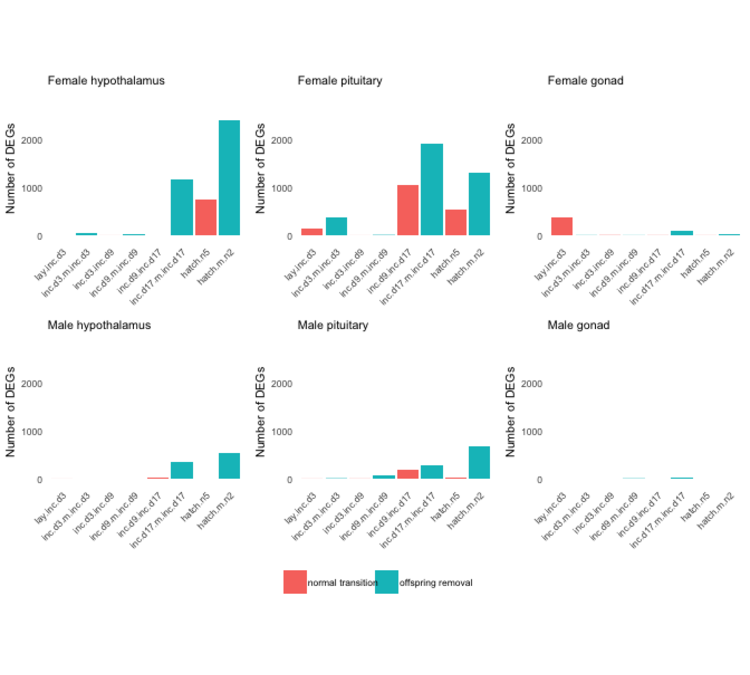
\includegraphics{manipulation_manuscript_files/figure-latex/unnamed-chunk-2-1.pdf}

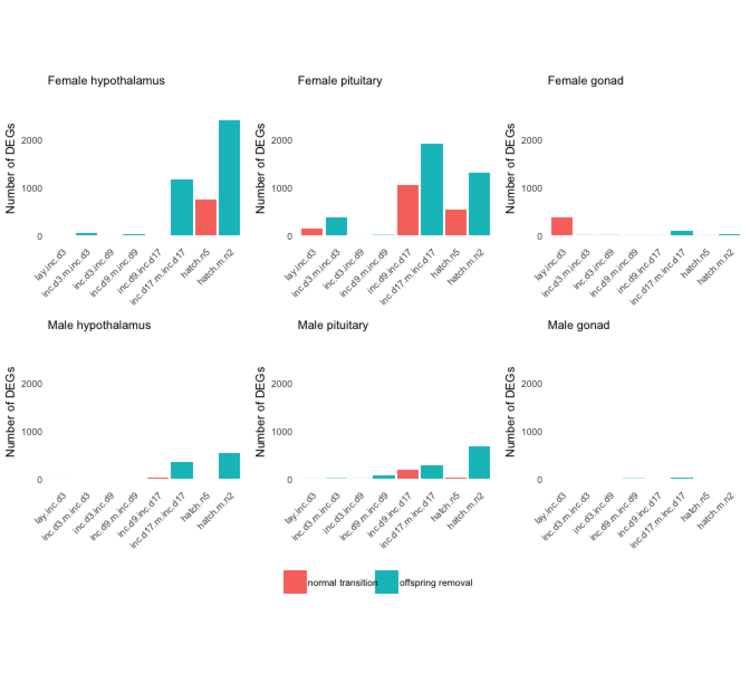
\includegraphics{manipulation_manuscript_files/figure-latex/unnamed-chunk-3-1.pdf}

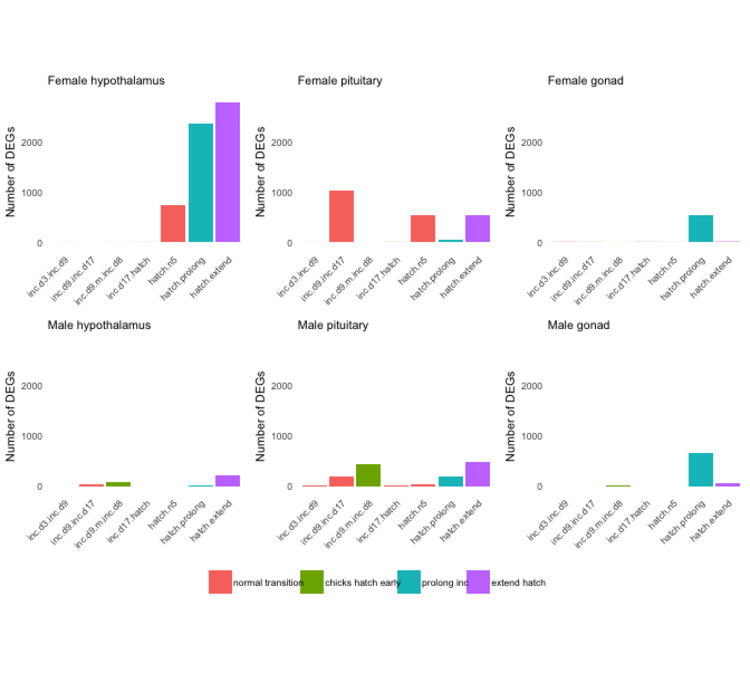
\includegraphics{manipulation_manuscript_files/figure-latex/unnamed-chunk-4-1.pdf}

\hypertarget{supplementary-figures}{%
\section{Supplementary Figures}\label{supplementary-figures}}

\hypertarget{acknowledgments}{%
\section{Acknowledgments}\label{acknowledgments}}

This project is a synergistic collaboration between the PI, Rebecca
Calisi-Rodríguez (expertise in avian behavior, parental care and
neurobiology), co-PI, Matthew MacManes (expertise in next-generation
sequencing, transcriptome assembly, and gene expression analyses), and
Collaborator, Rae Silver (expertise in neurobiology, dove behavior, and
decades of successful breeding and maintenance of dove colonies at
Barnard College).

\hypertarget{references}{%
\section*{References}\label{references}}
\addcontentsline{toc}{section}{References}

\nolinenumbers


\end{document}

